\chapter{Presentation of the activities carried out during the internship}
\label{sec:introduction}
\section{Presentation of objectives}
\label{sec:purpose}

The burnup of the fuel is one of the most important part in reactor simulation softwares,
while the depletion of the control rods
(which will also be called the \textit{burnup} of control rods in following sections, noted as $B_{cr}$)
is rarely considered.
In most cases, this will introduce no great error thanks to the short period of time
in which the control rods are inserted.
However, in rod-controlled small reactors,
where the period of insertion matches the life of the reactor,
such effect could no longer be neglected.

Recently, the development of a deterministic software in CGN requires such consideration.
The software requires calculating \textbf{the change in the fuel assembly's macroscopic cross section introduced by the insertion of control rods.}
This change is previously found to be mainly related to three factors: concentration of boron ($C_B$),
temperature of control rod ($T$) and density of moderator ($\rho$)
(Enrichment of \textit{U235} and the geometry are considered as fixed so are not included as variables.).
\begin{equation}
    \label{eq:DeltaSigma_no_cr}
    (\Delta\Sigma)^{cr} = f_0(C_B, T, \rho)
\end{equation}
The correlation $f_0$ was calculated by interpolation of a table of values.


It is found in a preliminary research
that the influence of the burnup of control rods is also related to these parameters.
So it is impossible to simply correct the correlation by simple manipulations like, for example,
adding a burnup correction factor.
\begin{equation}
    \label{eq:DeltaSigmaF}
    (\Delta\Sigma)^{cr} = f_0(C_B, T, \rho)F(B_{cr})
\end{equation}

The problem of this method is that this burnup correction factor is,
in addition to the burnup of control rods,
also related to the three parameters.
\begin{equation}
    \label{eq:burnup_correction_factor}
    F = f_F(C_B, T, \rho, B_{cr})
\end{equation}

So instead of correcting existing correlations, we could build directly new correlations that include $B_{cr}$.
\begin{equation}
    \label{eq:DeltaSigma}
    (\Delta\Sigma)^{cr} = f_1(C_B, T, \rho,B_{cr})
\end{equation}

This correlation could be calculated by building another table, or a new innovative method,
by training a deep neural network.
And it's the final objective to \textbf{obtain this correlation} in no matter which form.


\section{Presentation of the methods and procedures used}
\label{sec:methods}
\subsection{Software}
\label{sec:software}
The software chosen for Monte Carlo transport simulations is SERPENT which is specially designed for nuclear reactors.
It is developed by a Finnish research team in VTT technology research center based on continuous energy.
The version is 2.1.21 which is announced in June 2014.
It is very easy to perform burnup calculations in SERPENT without needs to couple extern solver.
Users need only to set up the burnup intervals and some normalization parameters to perform the calculations.
It is also very convenient to track the atom density change of nuclides since a mere configuration of the inventory is enough.
The output of the software is MATLAB scripts that could be read directly and manipulated easily in MATLAB.



\subsection{Model information}
\label{sec:model}
\paragraph{Model geometry}
\label{sec:geometry}

A typical fuel assembly consisting of $17\times17$ rods of a PWR is used.
No Gd rods are included. The guide tube in the center is filled with water.
Other guide tubes are filled with \textit{Ag-In-Cd} control rods.
Gaps in these rods are not considered except the water between control rod's
outer diameter and guide tube's inner diameter.
In order to take account of the self-shielding problem of control rods,
it is divided into 3 circles in burnup calculations.

Final geometry is shown in Fig \ref{fig:geo}.
The black triangle indicates the part that is defined explicitly in the model.
The other parts are generated using symmetries.
\begin{figure}[!htb]
    \centering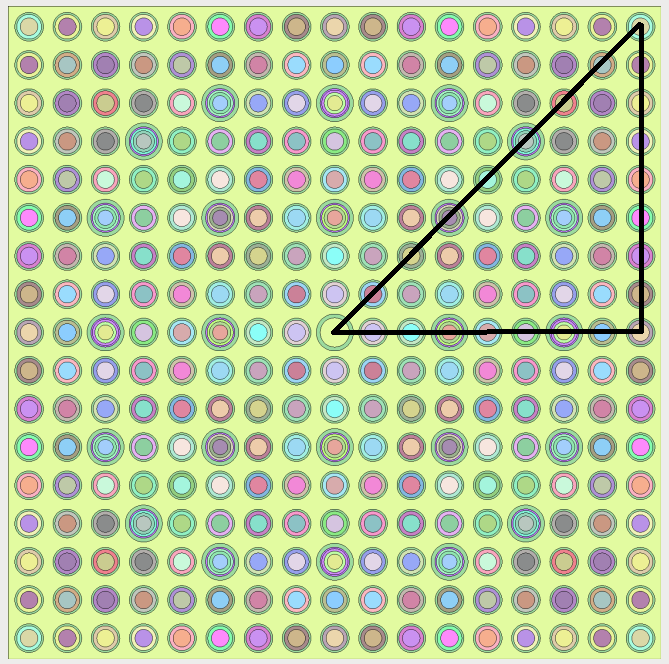
\includegraphics[width=0.5\linewidth]{Figs/model.png}
    \caption{Geometry drawn with Monte Carlo simulation software}
    \label{fig:geo}
\end{figure}


\paragraph{Material details}
\label{sec:material_details}
For the cladding of fuel rods and guide tubes, optimized ZIRLO is used.

For the cladding of control rods inside guide tubes, stainless steel type 304 is used.

\textit{Ag-In-Cd} alloy is used as the neutron absorber material for control rods.

Unless otherwise specified, water density is set to \textit{0.68 g/cc} with boron concentration 600 ppm.
Fuel enrichment is set to \textit{4.2\%}.
Fuel temperature is set to \textit{900 K}.
Moderator and other claddings' temperature is set to \textit{600 K}.
Power density is set to \textit{38.6 W/gU} for burnup calculations.



\subsection{Quantification of the burnup of control rods}
\label{sec:quantification_methods}

In order to research the effect of the burnup of control rods and further
include it in a Deep Neural Network.
It is necessary to find a physical quantity that could quantify the burnup of control rods.
This physical quantity will be noted as $ B_{cr} $ in the following sections.

The most direct one is the change in the sum of the product of the atom density
and the hot neutron absorption cross section of all nuclides in the control rod.
It represents the decrement of the control rods' ability to absorb hot neutrons.

\begin{equation}
    \label{eq:bcr0}
    B_{cr0} = \Delta \Sigma_i N_i \sigma_{h,i}
\end{equation}

where $N_i$ is the atom density of the nuclide and
$\sigma_{h,i}$ is the hot neutron absorption cross section of the nuclide.
However, this value cannot be directly read from many fuel assembly simulation softwares.
Then it is needed to find a physical quantity that is proportional to this quantity and
that one has easy access to in simulation softwares.

The fuel assembly's macro burnup is used as a mean to represent
the control rods' burnup in preliminary researches.
However, this method is not very reasonable since in different fuel assemblies,
the burnup of control rods could be very different as shown in Figure \ref{fig:bcr0-bu}.

\begin{figure}[!htb]
    \centering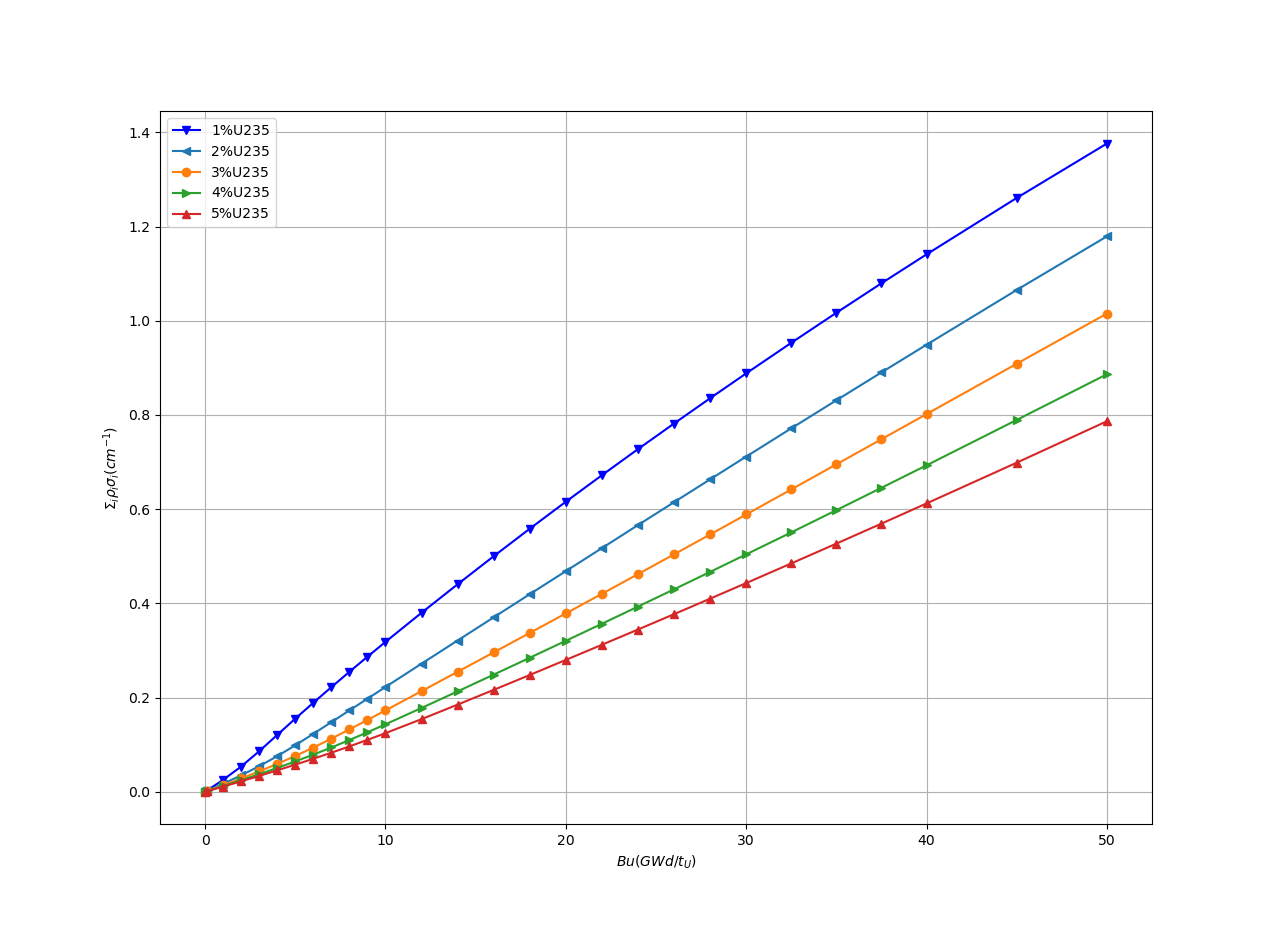
\includegraphics[width=0.6\linewidth]{Figs/Bcr0_Bu_difU.png}
    \caption{$B_{cr0}$ as a function of fuel burnup for different enrichments}
    \label{fig:bcr0-bu}
\end{figure}


In most softwares, for simplicity the neutron energy is divided into two groups.
One is the hot group (\textit{0-0.625 eV}) and the other is the fast group (higher than \textit{0.625 eV}).
So we propose the following quantity

\begin{equation}
    \label{eq:bcr}
    B_{cr} = \int_{\mathcal{T}}\phi_hdt + k\int_{\mathcal{T}}\phi_fdt
\end{equation}

where $\mathcal{T}$ is the set of time in which the control rods are irradiated,
$\phi_h,\phi_f$ are the average neutron flux density in the control rods
of hot group and fast group respectively.
And $k$ is called the \textit{hot-fast group proportion factor}.
By choosing the right $k$, one can prove that this $B_{cr}$ in equation \ref{eq:bcr}
is proportional to the $B_{cr0}$ in equation \ref{eq:bcr0}.

By dividing the neutron energy group to hot and fast group. We'll have
\begin{align*}
    B_{cr0} & = \Delta\Sigma_i \sigma_{h,i} N_i                                                                                           \\
            & = \Sigma_i \sigma_{h,i} \Delta N_i                                                                                          \\
            & = \Sigma_i \sigma_{h,i} N_i(\sigma_{h,i} \int_{\mathcal{T}}\phi_hdt + \sigma_{f,i}\int_{\mathcal{T}}\phi_fdt)               \\
            & = \Sigma_i \sigma_{h,i}^2 N_i \int_{\mathcal{T}}\phi_hdt + \Sigma_i \sigma_{h,i}\sigma_{f,i} N_i \int_{\mathcal{T}}\phi_fdt
\end{align*}

by noting $K = \Sigma_i \sigma_{h,i}^2 N_i $,
$k = \frac{\Sigma_i \sigma_{h,i}\sigma_{f,i} N_i}{K}$, we have
\begin{align}
    \label{eq:proved}
    \nonumber
    B_{cr0} & = K(\int_{\mathcal{T}}\phi_hdt + k\int_{\mathcal{T}}\phi_fdt) \\
            & = KB_{cr}
\end{align}

which proves the proportionality and the gives a method of calculating $k$.
The results will be shown in the results chapter(\ref{sec:quantification_results})
where the goodness of this quantification is evaluated.

\subsection{Neuron network setup}
\label{sec:neuron_network_setup}
\paragraph{Prefix}
\label{sec:dnn_pre}
In many circumstance, traditional methods use tables and interpolation to estimate
multi-variable non-linear functions.
Either because the correlation is too complicated to calculate or
no explicit correlation could be obtained at all.
In our case, the relation between the change in the macroscopic cross section of
fuel assembly introduced by insertion of control rods and $(C_B, T, \rho, B_{cr})$ is later.
No explicit correlations exist and regressions are difficult to carry out.

Machine learning is a very hot topic in recent years.
It has changed the way people work in many fields, like picture recognizing or auto-mobile.
Although this is not its main field of usage,
it provides very good methods for regressions of multi-variable non-linear functions.
The Universality Theorem proves that any continuous function with a finite number of inputs in
a finite range can be approached as precisely as wanted
by a single hidden layer neuron network with sufficient number of neurons
with specific activation functions.
This is the common case for functions in physics.
This ensures that in our situation, it is possible to apply deep neuron network.

\paragraph{Data acquisition}
\label{sec:dnn_data}
At first, the material cards of control rods at different burnup($B_{cr}$) are prepared by tracking
atom density change and linking it to calculated $B_{cr}$.
In this part, fuel burnup intervals are set to be very small to provide precise materials.
There are 50 intervals between \textit{0} and \textit{50 GWd/tU} burnup.
In fact, since the atom densities change nearly linearly as shown in section \ref{sec:material},
interpolation will give very precise results in points other than these 50.

\begin{table}[!htb]
    \caption{Parameter range and normalization formula}
    \label{tab:norm}
    \centering
    \begin{tabular}{l l l l}
        \hline
        \textbf{variable} & \textbf{range} & \textbf{Unit}                & \textbf{formula}                 \\
        \hline
        $C_B$             & [0, 3000]      & \textit{ppm}                 & $C_B = n \times 3$               \\
        $T$               & [300, 900]     & \textit{K}                   & $T = 300 + n \times 0.6$         \\
        $\rho$            & [0.6, 1.0]     & \textit{g/cc}                & $\rho = 0.6 + n \times 0.0004$   \\
        $B_{cr}$          & [0.0, 8.6]     & \textit{$10^{18}$ $cm^{-1}$} & $B_{cr} = n \times 8.6.10^{18} $ \\
        \hline
    \end{tabular}
\end{table}
Then a number $N$ of random couples of $(C_B, T, \rho, B_{cr})_n$ are generated in range [0, 1000].
Real values $(C_B, T, \rho, B_{cr})$ can be calculated by the formula given in Table \ref{tab:norm}.
Simulations show that $\Sigma^{cr}$ changes very fast in range [0.0, 1.7] \textit{$10^{18}$ $cm^{-1}$}
(for normalized value [0, 200]) and much slower after.
So in order to improve the efficiency of neuron network, values for $B_{cr}$ are not chosen completely randomly
but follows a Gaussian distribution whose mean value is \textit{0} and standard deviation is \textit{200}.
We take the absolute values of this set of Gaussian distribution and
values that exceeds \textit{1000} are taken care of by a modulo operation.

Corresponding material cards are generated and put in the model described at \ref{sec:model}.
Then two calculations are performed.
One with all control rods inserted and we could get a macroscopic hot neutron absorption cross section $\Sigma^{cr}$.
The other one with no control rods inserted and we get $\Sigma^{no\_cr}$.
The change in macroscopic cross section is then calculated by
\begin{equation}
    \label{eq:dSigma}
    \Delta \Sigma^{cr} = \Sigma^{cr} - \Sigma^{no\_cr}
\end{equation}

The $\Delta \Sigma^{cr}$ is also normalized to [0, 1000]
by setting the minimal to \textit{0} and maximal to \textit{1000}.
By this method, we'll get $N$ sets of $(\Delta \Sigma^{cr}, C_B, T, \rho, B_{cr})_n$ which
could be used for training a neuron network.



\paragraph{Neuron network details}
\label{sec::dnn_para}

We use TensorFlow.Keras to construct our neuron network for simplicity.
TensorFlow is a mathematical Python library designed for building machine learning models.
The version we used is \textit{2.0.0}.
Keras is now a submodule of TensorFlow that is very convenient for building simple neuron networks
for general purposes.
Setup of a model requires only several configurations of parameters,
with no explicit design of the model required.
In our model, only the most basic parameters need to be configured.

At the beginning, all the data are divided to two sets.
One for training the model which takes \textit{80\%} data and
the other for testing which takes the remaining \textit{20\%} data.
Then all input will be divided by \textit{1000} (range shrunk to [0, 1]) which is a
standard normalized data range for neuron networks.
Output values are between [0, 1000] which remain unchanged.

\textit{Keras Sequential} is a good model for regressions, we add two dense layers with 2048 neurons each.
In order to avoid overfitting problem, an early-stop function is defined.
The function will monitor \textit{var\_loss} variable (the loss of network on the test data set) to
detect if overfitting exists and stop the training as soon as the early-stop criteria is satisfied.


After the training is finished, \textit{mean absolute error} is calculated on test data set to evaluate the
goodness of the model.

